\documentclass{beamer}

\usepackage[utf8]{inputenc}
\usepackage{utopia}            % font utopia imported
\usepackage{amsmath}
\usepackage{latexsym}
\usepackage{calc}              % support command '\widthof'
\usepackage{xcolor}            % support multiple color 
\usepackage{arydshln}
\usepackage{amssymb}  
\usepackage{booktabs}
\usepackage{graphicx}
\usepackage{subcaption}
\usepackage{bookmark}
\usepackage{float}
\usepackage{bm}
\usepackage{bbold}
\usepackage{extarrows}

\usefonttheme{professionalfonts} 

\makeatletter
\let\@@magyar@captionfix\relax
\makeatother

\usetheme{Madrid}
\usecolortheme{default} 

%======================================================================%
\title[CMT.Tsinghua]{Introduction to Magnetic Exchange Mechanisms}

\subtitle{(From Heisenberg model to Goodenough-Kanamori rule)}

\author[Yang Li]
{Yang Li\inst{1}}  

\institute[Physics@Tsinghua] 
{
  \inst{1}%
  Department of Physics\\
  Tsinghua University 
}

\date[Tsinghua Physics 2020]{May. 2020}
%======================================================================

%======================================================================
\AtBeginSection[]
{
  \begin{frame}
    \frametitle{Table of Contents}
    \tableofcontents[currentsection]
  \end{frame} 
}
%======================================================================
 
\begin{document}
  %======================================================================
  \frame{\titlepage}
  %======================================================================

  %======================================================================
  \begin{frame}
    \frametitle{Table of Contents}
    \tableofcontents
  \end{frame}
  %======================================================================

  \section{Two Spin Sites Model}

  %======================================================================
  \begin{frame}
    \frametitle{Spin space for two spin sites}
    For a \textcolor{purple}{two equivalent spin-\(\frac{1}{2}\) spin sites} (a and b), the complete spin space can be described by 4 states:
    \begin{equation*}
      \begin{aligned}
        &|\uparrow,\uparrow\rangle, |\downarrow,\downarrow\rangle \;\;\;\text{ferromagnetic(FM) states}\\
        &|\uparrow,\downarrow\rangle, |\downarrow, \uparrow\rangle \;\;\;\text{anti-ferromagnetic (AFM) states}
      \end{aligned}
    \end{equation*}

    The eigenstates for a spin coupling system can be produced by the linear combination of those 4 states.
    \begin{equation*}
      \begin{aligned}
        &\left.\begin{aligned}|1,1\rangle &= |\uparrow,\uparrow\rangle\\
        |1,-1\rangle &= |\downarrow,\downarrow\rangle\\
        |1,0\rangle &= \frac{1}{\sqrt{2}}\left(|\uparrow,\downarrow\rangle + |\downarrow, \uparrow\rangle\right) \end{aligned}\right\} \text{triplet states for}\; s = 1\\
        &\;\;\;\;|0,0\rangle = \frac{1}{\sqrt{2}}\left(|\uparrow,\downarrow\rangle - |\downarrow, \uparrow\rangle\right)\;\;\; \text{singlet state for}\; s = 0
      \end{aligned}
    \end{equation*}
  \end{frame}
  %====================================================================== 

  %======================================================================
  \begin{frame}
    \frametitle{The origin of magnetism}
    Assume the energy of the spin triplet states are degenerated. Use \(E_\text{T}
    \) and \(E_\text{S}\) represent the energy of \textcolor{purple}{the spin triplet and spin singlet states}, respectively.
    \begin{equation}
      \begin{aligned}
        E_{\text{FM}} - E_{\text{AFM}} &= E_{\uparrow,\uparrow} - E_{\downarrow,\uparrow}\\
        &= E_{\uparrow,\uparrow} - E_{\uparrow,\downarrow}\\
        &= E_{1,1} - \frac{1}{2}E_{1,0} - \frac{1}{2}E_{0,0}\\
        &= \frac{1}{2}(E_\text{T} - E_\text{S})
      \end{aligned}
    \end{equation}
    \begin{block}{Mark}
      Obviously, the AFM state and the spin singlet state are different. But, once we express the \(E_\text{T} - E_\text{S}\) using the spin order, naturaly, the \(E_{\text{FM}} - E_{\text{AFM}}\) will also be included.
    \end{block}
  \end{frame}
  %====================================================================== 

  %======================================================================
  \begin{frame}
    \frametitle{Heisenberg Hamiltonian for two spin sites}
    Let \(E_\text{T} - E_\text{S} = -2A\), more specifically, \(E_\text{T} = -A, E_\text{S} = A\) \textcolor{gray}{(If not, just give it an energy shift)}.
    
    At the same time, for the two spin operators \(\widehat{\bm{s}}_1, \widehat{\bm{s}}_2\), 
    \begin{equation}
      \begin{aligned}
        2\langle\widehat{\bm{s}}_1\cdot\widehat{\bm{s}}_2\rangle + \frac{1}{2} &= s(s+1) - s_1^2 - s_2^2 + \frac{1}{2} \\
        &= \begin{cases}
          -1, s = 0\\
          +1, s = 1 
        \end{cases}
      \end{aligned}
    \end{equation}
    Where \(\widehat{\bm{s}} = \widehat{\bm{s}}_1+\widehat{\bm{s}}_2\), and the unit \(\hbar\) is not included.
    \begin{block}{Important Result}
      So, the Hamiltonian for \(E_\text{T}\) and \(E_\text{S}\) can be written as:
    \begin{equation}
      \widehat{H}_{A\text{d}} = -2A\;\widehat{\bm{s}}_1\cdot\widehat{\bm{s}}_2
    \end{equation}
    This is what we called, Heisenberg Hamiltonian \textcolor{gray}{(for two spin sites)}.
    \end{block}
  \end{frame}
  %====================================================================== 
  
  \section{Coefficient \(A\) in Heisenberg Model}

  %======================================================================
  \begin{frame}
    \frametitle{A naive idea about the origin of \(A\) --- MDD}
    The only question now is the origin of the coefficient \(A\).
    \begin{block}{Naive idea}
      Since the Heisenberg Hamiltonian is directly related to spin, it is nature to think that the \(A\) may come from spin-spin interaction. Or more specifically, it comes from the magnetic dipole-dipole(MDD) interaction.
    \end{block}
    The magnetic dipole generated by spin can be calculated as follow:
    \begin{equation}
      \bm{\mu}_S = -g_e\mu_{\text{B}}\langle\widehat{\bm{S}}\rangle
    \end{equation}
    Dirac theory gives \(g_e = 2\), which is changed to \(g_e\approx2.0023\) by QED corrections.
  \end{frame}
  %======================================================================

  %======================================================================
  \begin{frame}
    \frametitle{A naive idea about the origin of \(A\) --- MDD}
    \begin{block}{Useful energy scales}
      \begin{itemize}
        \item \(1\;\text{T} \sim 5.8\times10^{-2}\;\text{meV} \sim 0.67\;\text{K}\)
        \item \(1\;\text{meV} \sim 11.6\;\text{K} \sim 17.2\;\text{T} \sim 8.06\;\text{cm}^{-1}\)
        \item \(1\;\text{cm}^{-1} \sim 1.44\;\text{K}\)
      \end{itemize}
    \end{block}
    The energy magnetic dipole-dipole interaction can be calculate by:
      \begin{equation}
        E_{\text{mdd}} = \dfrac{\mu_0}{4\pi} \dfrac{\bm{\mu_1}\cdot\bm{\mu_2} - 3(\bm{e}_R\cdot\bm{\mu_1})(\bm{e}_R\cdot\bm{\mu_2})}{R^3}
      \end{equation}

    \begin{block}{Estimate \(T_\text{C}\) under MDD}
      For two \(1\;\mu_{\text{B}}\) moments at a distance of \(1\;\text{\AA}\) the magnetostatic energy is of the order of \(0.05\) meV, corresponding to a temperature of less than \(1\) K. 
    \end{block}
    While, The \(T_\text{C}\) for Fe\(_3\)O\(_4\) is \(858\) K.
  \end{frame}
  %======================================================================

  %======================================================================
  \begin{frame}
    \frametitle{Three methods to obtain the coefficient \(A\)}
    The real source of \(A\) is the electron exchange, a quantum many-body interaction. 
    
    There are three ways (as I konw) to get coefficient \(A\). Each of them uniquely help us understand the origin of magnetic order.
    \begin{block}{Preview for the 3 method}
      \begin{itemize}
        \item The first method can help us understand the essence of \(A\).
        \item The second method teach us how to determine the sign of \(A\), and gives a more clear descripution about \(A\).
        \item As for the last one, we can use it in the daily research.
      \end{itemize}
    \end{block}
  \end{frame}
  %======================================================================

  %======================================================================
  \begin{frame}
    \frametitle{The 1st method \(\blacktriangleright\) Hamiltonian}
    The first and the directest \textcolor{gray}{(also the earliest)} method is given by \textcolor{purple}{Heitler and London}\footnote{Physik, 1927,44,455} using hydrogen molecule. 

    In a hydrogen molecule, assume each hydrogen site has one electron without inter-site hopping. Then, the Hamiltonian for this system is,
    \begin{equation}
      \begin{aligned}
        \widehat{H}_{\text{h}} &= -\dfrac{\hbar^2}{2m}\left(\nabla_1^2 + \nabla_2^2\right) - \dfrac{e^2}{r_{a1}} - \dfrac{e^2}{r_{b2}} + \dfrac{e^2}{R_{ab}} + \dfrac{e^2}{r_{12}} - \dfrac{e^2}{r_{b1}} - \dfrac{e^2}{r_{a2}}\\
        &= \widehat{H}_{01} + \widehat{H}_{02} + \dfrac{e^2}{R_{ab}} + \widehat{H}_U - \dfrac{e^2}{r_{b1}} - \dfrac{e^2}{r_{a2}}
      \end{aligned}
    \end{equation}
    \begin{columns}
      \begin{column}{0.6\textwidth}
        Where {\small \(\widehat{H}_{01} = -\dfrac{\hbar^2}{2m}\nabla_1^2 - \dfrac{e^2}{r_{a1}}\), \\
    \ \ \ \ \ \ \ \ \ \(\widehat{H}_{02} = -\dfrac{\hbar^2}{2m}\nabla_2^2 - \dfrac{e^2}{r_{b2}}\), \\
    \ \ \ \ \ \ \ \ \ \(\widehat{H}_U = \dfrac{e^2}{r_{12}}\)}.
      \end{column}
      \begin{column}{0.35\textwidth}
      \end{column}
    \end{columns}
  \end{frame}
  %======================================================================

  %======================================================================
  \begin{frame}
    \frametitle{The 1st method \(\blacktriangleright\) Basis}
    \begin{equation*}
        \widehat{H}_{\text{h}} = \widehat{H}_{01} + \widehat{H}_{02} + \dfrac{e^2}{R_{ab}} + \widehat{H}_U - \dfrac{e^2}{r_{b1}} - \dfrac{e^2}{r_{a2}}
    \end{equation*}
    Use the eigenstates of \(\widehat{H}_{01} + \widehat{H}_{02}\) to describe the low energy part of the Hilbert space. After consider the symmetry for fermion, 
    \begin{equation}
      \begin{cases}
        \psi_{\text{S}} &= \frac{1}{\sqrt{2}}\left[\psi_a(1)\psi_b(2) + \psi_a(2)\psi_b(1)\right]\\
        \psi_{\text{T}} &= \frac{1}{\sqrt{2}}\left[\psi_a(1)\psi_b(2) - \psi_a(2)\psi_b(1)\right]
      \end{cases}
    \end{equation}
    Under this basis, the \(\widehat{H}_{\text{h}}\) can be expressed as:
    \begin{equation}
      \widehat{H}_{\text{h}} = 2E_0 + \dfrac{e^2}{R_{ab}} + \begin{pmatrix}
        \frac{K+A}{1+I^2} & 0 \\
        0 & \frac{K-A}{1-I^2}\\
      \end{pmatrix}, \;\;\begin{pmatrix}
        \psi_{\text{S}}\\[0.6em]
        \psi_{\text{T}}
      \end{pmatrix}
    \end{equation}
  \end{frame}
  %======================================================================

  %======================================================================
  \begin{frame}
    \frametitle{The 1st method \(\blacktriangleright\) Energy difference}
    \begin{equation*}
      \widehat{H}_{\text{h}} = 2E_0 + \dfrac{e^2}{R_{ab}} + \begin{pmatrix}
        \frac{K+A}{1+I^2} & 0 \\
        0 & \frac{K-A}{1-I^2}\\
      \end{pmatrix} \ \ \ \begin{matrix}
        |\psi_{\text{S}}\rangle\\[0.5em]
        |\psi_{\text{T}}\rangle
      \end{matrix}
    \end{equation*}
    Where,
    \begin{subequations}
      \begin{align}
        K &= \int \psi_a^*(1)\psi_b^*(2)\left(\dfrac{e^2}{r_{12}} - \dfrac{e^2}{r_{b1}} - \dfrac{e^2}{r_{a2}}\right)\psi_a(1)\psi_b(2)\;\mathrm{d}^3r_1\mathrm{d}^3r_2\\
        A &= \int \psi_a^*(1)\psi_b^*(2)\left(\dfrac{e^2}{r_{12}} - \dfrac{e^2}{r_{b1}} - \dfrac{e^2}{r_{a2}}\right)\psi_a(2)\psi_b(1)\;\mathrm{d}^3r_1\mathrm{d}^3r_2\\
        I^2 &= \int \psi_a^*(1)\psi_b^*(2)\psi_a(2)\psi_b(1)\;\mathrm{d}^3r_1\mathrm{d}^3r_2
      \end{align}
    \end{subequations}
    Since \(I^2 \ll 1\), \(E_\text{T} - E_\text{S} \approx -2A\) \qed
  \end{frame}
  %======================================================================

  %======================================================================
  \begin{frame}
    \frametitle{The 2nd method \(\blacktriangleright\) Hamiltonian}
    \begin{equation*}
      \begin{aligned}
        \widehat{H}_{\text{h}} &= -\dfrac{\hbar^2}{2m}\left(\nabla_1^2 + \nabla_2^2\right) - \dfrac{e^2}{r_{a1}} - \dfrac{e^2}{r_{b2}} + \dfrac{e^2}{R_{ab}} + \dfrac{e^2}{r_{12}} - \dfrac{e^2}{r_{b1}} - \dfrac{e^2}{r_{a2}}\\
        &= \widehat{h}_{1} + \widehat{h}_{2} + \dfrac{e^2}{R_{ab}} + \widehat{H}_U 
      \end{aligned}
    \end{equation*}
    \begin{columns}
      \begin{column}{0.7\textwidth}
        Where {\small \(\widehat{h}_{1} = -\dfrac{\hbar^2}{2m}\nabla_1^2 - \dfrac{e^2}{r_{a1}} - \dfrac{e^2}{r_{b1}}\), \\
        \ \ \ \ \ \ \ \ \ \(\widehat{h}_{2} = -\dfrac{\hbar^2}{2m}\nabla_2^2 - \dfrac{e^2}{r_{a2}} - \dfrac{e^2}{r_{b2}}\)}.\\[0.5em]
        The introduce of \(\widehat{h}_{1}\) (or \(\widehat{h}_{2}\)) lead us to the bonding state and the anti-bonding state.
        \begin{subequations}\small
          \begin{align}
            \phi_1 &= \dfrac{1}{\sqrt{2(1+I^2)}}(\psi_a+\psi_b) \approx \dfrac{1}{\sqrt{2}}(\psi_a+\psi_b)\\
            \phi_2 &= \dfrac{1}{\sqrt{2(1-I^2)}}(\psi_a-\psi_b) \approx \dfrac{1}{\sqrt{2}}(\psi_a-\psi_b)
          \end{align}
        \end{subequations}
      \end{column}
      \begin{column}{0.25\textwidth}
      \end{column}
    \end{columns}
    
  \end{frame}
  %======================================================================

  %======================================================================
  \begin{frame}
    \frametitle{The 2nd method \(\blacktriangleright\) Ground state}
    The energy difference between \(\phi_1\) and \(\phi_2\) is denoted as: \(\Delta = E_2 - E_1\).

    Accroding to symmetry, there are 3 different kind of electron occupation. 
    \begin{equation*}
      \begin{matrix}
      \phi_2&\ \ \overline{\hspace{4em}}\ \ &\ \ \overline{\hspace{4em}}\ \ &\ \ \overline{\hspace{4em}}\ \ \\[0.6em]
      \phi_1&\ \ \overline{\hspace{4em}}\ \ &\ \ \overline{\hspace{4em}}\ \ &\ \ \overline{\hspace{4em}}\ \ \\[0.6em]
      \ &\Phi_{\text{T}}&\Phi_{\text{S}1}&\Phi_{\text{S}2}
      \end{matrix}
    \end{equation*}
     
    The ground state for spin triplet: \(\Phi_{\text{T}}\).\\
    The ground state for spin singlet: \(\Phi_{\text{S}} = \lambda_1 \Phi_{\text{S}1} + \lambda_2 \Phi_{\text{S}2}\).

    Use these two state, we can calculate the energy difference between spin triplet and singlet state\footnote{J. Am. Chem. Soc. 1975,97,17,4884}:
    \begin{equation}
      -2A = E_\text{T} - E_\text{S} = -2J_{ab} + \dfrac{\Delta^2}{U}
    \end{equation}
  \end{frame}
  %======================================================================

  %======================================================================
  \begin{frame}
    \frametitle{The 2nd method \(\blacktriangleright\) Energy difference}
    \begin{equation*}
      -2A = E_\text{T} - E_\text{S} = -2J_{ab} + \dfrac{\Delta^2}{U}
    \end{equation*}
    Where,
    \begin{subequations}
      \label{eq::defJU}
      \begin{align}
        J_{ab} &= \int \psi_a^*(1)\psi_b^*(2)\dfrac{e^2}{r_{12}}\psi_a(2)\psi_b(1)\;\mathrm{d}^3r_1\mathrm{d}^3r_2\\
        U_{ij} &= \int \psi_i^*(1)\psi_j^*(2)\dfrac{e^2}{r_{12}}\psi_i(1)\psi_j(2)\;\mathrm{d}^3r_1\mathrm{d}^3r_2\\
        U &= U_{aa} - U_{ab}
      \end{align}
    \end{subequations}
   \textcolor{gray}{In the first method, we get:
   \begin{equation*}
    A = \int \psi_a^*(1)\psi_b^*(2)\left(\dfrac{e^2}{r_{12}} - \dfrac{e^2}{r_{b1}} - \dfrac{e^2}{r_{a2}}\right)\psi_a(2)\psi_b(1)\;\mathrm{d}^3r_1\mathrm{d}^3r_2
   \end{equation*}}
  \end{frame}
  %======================================================================

  %======================================================================
  \begin{frame}
    \frametitle{The 2nd method \(\blacktriangleright\) The sign of \(J_{ab}\)}
    \begin{equation}
      \begin{aligned}
        J_{ab} &= \int \psi_a^*(1)\psi_b^*(2)\dfrac{e^2}{r_{12}}\psi_a(2)\psi_b(1)\;\mathrm{d}^3r_1\mathrm{d}^3r_2\\
        &= \int \mathrm{d}^3r_1 \underbrace{\psi_a^*(1)\psi_b(1)}_{\Psi^*(1)} \int \mathrm{d}^3r_2 \dfrac{e^2}{|\bm{r_1} - \bm{r_2}|}\underbrace{\psi_a(2)\psi_b^*(2)}_{\Psi(2)}\\
        &= \int \mathrm{d}^3r_1\; \Psi^*(1) \dfrac{1}{(2\pi)^3}\int \mathrm{d}^3k\; \mathrm{e}^{i\bm{k}\cdot\bm{r_1}} \dfrac{4\pi}{k^2} \widetilde{\Psi}(\bm{k})\\
        &= \dfrac{1}{(2\pi)^3}\int \mathrm{d}^3k\; \underbrace{\int \mathrm{d}^3r_1\; \mathrm{e}^{i\bm{k}\cdot\bm{r_1}}\Psi^*(1)}_{\widetilde{\Psi}^*(-k)} \widetilde{\Psi}(\bm{k})\dfrac{4\pi}{k^2}\\
        &= \dfrac{1}{(2\pi)^3}\int \mathrm{d}^3k\; \left|\widetilde{\Psi}(\bm{k})\right|^2\dfrac{4\pi}{k^2} > 0 
      \end{aligned}
    \end{equation}
  \end{frame}
  %======================================================================

  %======================================================================
  \begin{frame}
    \frametitle{The 2nd method \(\blacktriangleright\) Useful observations}
    \begin{equation*}
      -2A = E_\text{T} - E_\text{S} = -2J_{ab} + \dfrac{\Delta^2}{U}
    \end{equation*}
    \begin{block}{Observations}
      \begin{itemize}
        \item The first term, \(J_{ab}\) is corresponding to the FM state. While, the second term, \(\Delta^2/U\) is corresponding to the AFM state.
        \item \textcolor{purple}{\(J_{ab}\) comes from the electron-electron Coulomb exchange.}
        \item \(\Delta^2/U\) comes from the electron-ion Coulomb interaction.
        \item \textcolor{purple}{\(\Delta^2/U\) can also be regard as the result of electron hopping in different atomic site. And \(\Delta = 2t\), where \(t\) is the hopping factor.}
        \item The \(\Delta\) here, is the origin of superexchange (or super-superexchange).
      \end{itemize}
    \end{block}
  \end{frame}
  %======================================================================

  %======================================================================
  \begin{frame}
    \frametitle{The 3rd method \(\blacktriangleright\) Starting point}
    \begin{block}{Starting Point}
      From the result of 2nd method, we can conclude that, the magnetic state energy difference comes from 2 sources: 
      \begin{itemize}
        \item The electron-electron Coulomb exchange. (\(-2J_{ab}\)) 
        \item Elelctron hopping among different sites. (\(4t^2/U\))
      \end{itemize} 
      And that encourage us to introduce the electron hopping in our system.
    \end{block}
    \begin{equation*}
      -2A = E_\text{T} - E_\text{S} = -2J_{ab} + \dfrac{4t^2}{U}
    \end{equation*}
    Remeber, in the \textcolor{purple}{first method} we declare that, the two electron in different site \textcolor{purple}{cannot hopping} to each other. Although, based on that assumption, we bulit up a \textcolor{purple}{complete Hilbert space} for ground state, but it is actually \textcolor{purple}{unphysical}. \textcolor{gray}{(It is hard to obtain some physical meaning from a Hamiltonian diagonalization.)}
  \end{frame}
  %======================================================================

  %======================================================================
  \begin{frame}
    \frametitle{The 3rd method \(\blacktriangleright\) Basic idea}
    Now, Let's open the black box of Hamiltonian diagonalization!
    \begin{block}{Basic idea}
      In the third method, we will still use the single electron state \(\psi_a, \psi_b\), but permit the electron hopping. That means, the two electrons are now permited to occupy the same site.
    
      Accroding to the analysis above, the energy different comes from two terms, which we named:
      \begin{itemize}
        \item Coulomb exchange
        \item Kinetic exchange
      \end{itemize}
    \end{block}
    \textcolor{gray}{The ``Coulomb exchange'' represent the electron-electron Coulomb exchange. We do not care about the Coulomb exchange when the two electrons occupy the same site, which is also in a independent space. So, when discussing the Coulomb exchange, there is no need to imply the hopping picture.}
  \end{frame}
  %======================================================================

  %======================================================================
  \begin{frame}
    \frametitle{The 3rd method \(\blacktriangleright\) Coulomb exchange}
    The Coulomb exchange is related to the electron-electron Coulomb interaction:
    \begin{equation}
      \widehat{H}_U = \dfrac{e^2}{r_{12}}
    \end{equation}
    In the first method, we use the spin singlet and triplet state to symmetrize the real space wavefunction. This work can also be done by one equation:
    \begin{equation}
      \begin{aligned}
        \Psi_{a,\sigma;b,\sigma'} &= \frac{1}{\sqrt{2}}\begin{vmatrix}
          \psi_a(1)\sigma(1) & \psi_a(2)\sigma(2)\\
          \psi_b(1)\sigma'(1) & \psi_b(2)\sigma'(2)
        \end{vmatrix}\\
        &= \frac{1}{\sqrt{2}}[\psi_a(1)\psi_b(2)\sigma(1)\sigma'(2) - \psi_b(1)\psi_a(2)\sigma'(1)\sigma(2)]
      \end{aligned}
    \end{equation}
    Where the \(\sigma\) and \(\sigma'\) is the single electron spin. 

    Instand of using the coupling representation, we express the \(\widehat{H}_U\) under the \textcolor{purple}{uncoupling representation}. 
  \end{frame}
  %======================================================================

  %======================================================================
  \begin{frame}
    \frametitle{The 3rd method \(\blacktriangleright\) Coulomb exchange}
    \begin{equation}
      \widehat{H}_U = \begin{pmatrix}
        U_{ab} - J_{ab} & 0 & 0 & 0\\
        0 & U_{ab} & -J_{ab} & 0 \\
        0 & -J_{ab} & U_{ab} & 0 \\
        0 & 0 & 0 & U_{ab} - J_{ab}
      \end{pmatrix}\ \ \ \begin{matrix}
        |\uparrow,\uparrow\rangle\\
        |\uparrow,\downarrow\rangle\\
        |\downarrow,\uparrow\rangle\\
        |\downarrow,\downarrow\rangle\\
      \end{matrix}
    \end{equation}
  \textcolor{gray}{Check equation \eqref{eq::defJU} to confirm the defination of \(U_{ab}\) and \(J_{ab}\).}
    \begin{block}{Observations}
      \begin{itemize}
        \item Coulomb exchange for spin triplet state: \(E_{\text{CT}} = U_{ab} - J_{ab}\).
        \item Coulomb exchange for spin singlet state: \(E_{\text{CS}} = U_{ab} + J_{ab}\).
        \item Under the Coulomb exchange, the state \(|\uparrow,\downarrow\rangle\) and \(|\downarrow,\uparrow\rangle\) are coupled. (This the basis of double exchange.)
        \item The Coulomb exchange always prefer spin triplet state, for the \(J_{ab}\) keep positive. 
      \end{itemize}
    \end{block}
  \end{frame}
  %======================================================================

  %======================================================================
  \begin{frame}
    \frametitle{The 3rd method \(\blacktriangleright\) Kinetic exchange \(\blacktriangleright\) Hubbard model}
    The kinetic exchange is related to the hopping of electrons. To describe this this part, we need to use the Hubbard model.
    \begin{equation}
      \widehat{H}_{t-U} = -t \sum_{ij\sigma}\widehat{c}^{\;\dagger}_{j\sigma}\widehat{c}_{i\sigma} + U \sum_i \widehat{n}_{i\uparrow}\widehat{n}_{i\downarrow}
    \end{equation}
    The \textcolor{purple}{spin parallel state} forbiden the electron hopping, so their kinetic energy \textcolor{purple}{equals to 0}.

    Under the basis: \(\{\;\overbrace{|\uparrow\cdot,\downarrow\cdot\rangle,|\downarrow\cdot,\uparrow\cdot\rangle}^{\text{covalent states}},\;\overbrace{|\uparrow\downarrow,\cdot\hspace{0.2em}\cdot\rangle,|\cdot\cdot,\uparrow\downarrow\rangle}^{\text{ionic states}}\;\}\),
    
    The Hamiltonian can be expressed as:
    \begin{equation}
      \widehat{H}_{t-U} = \begin{pmatrix}
        0 &  0 & -t & -t \;\\
        0 &  0 & +t & +t \;\\
       -t & +t &  U &  0 \;\\
       -t & +t &  0 &  U \;
      \end{pmatrix}\ \ \ \begin{matrix}
        |\uparrow\cdot,\downarrow\cdot\rangle\\
        |\downarrow\cdot,\uparrow\cdot\rangle\\
        |\uparrow\hspace{0.15em}\downarrow,\cdot\hspace{0.4em}\cdot\rangle\\
        |\hspace{0.1em}\cdot\hspace{0.15em}\cdot,\uparrow\hspace{0.15em}\downarrow\rangle
      \end{matrix}
    \end{equation}
  \end{frame}
  %======================================================================

  %======================================================================
  \begin{frame}
    \frametitle{The 3rd method \(\blacktriangleright\) Kinetic exchange \(\blacktriangleright\) Energy split}
    \begin{equation*}
      \widehat{H}_{t-U} = \begin{pmatrix}
        0 &  0 & -t & -t \;\\
        0 &  0 & +t & +t \;\\
       -t & +t &  U &  0 \;\\
       -t & +t &  0 &  U \;
      \end{pmatrix}\ \ \ \begin{matrix}
        |\uparrow\cdot,\downarrow\cdot\rangle\\
        |\downarrow\cdot,\uparrow\cdot\rangle\\
        |\uparrow\hspace{0.15em}\downarrow,\cdot\hspace{0.4em}\cdot\rangle\\
        |\hspace{0.1em}\cdot\hspace{0.15em}\cdot,\uparrow\hspace{0.15em}\downarrow\rangle
      \end{matrix}
    \end{equation*}
    After diagonalization, we get:
    \begin{subequations}\scriptsize
      \begin{align}
        &\varepsilon_+ = \dfrac{U}{2} + \dfrac{\sqrt{U^2+16t^2}}{2},\ \  \Psi_+ = \dfrac{|\uparrow\cdot,\downarrow\cdot\rangle - |\downarrow\cdot,\uparrow\cdot\rangle - (\varepsilon_+/2t)(|\uparrow\downarrow,\cdot\hspace{0.2em}\cdot\rangle + |\cdot\cdot,\uparrow\downarrow\rangle)}{\sqrt{2+(\varepsilon_+/2t)^2}}\\
        &\varepsilon_{\text{ion}} = U,\hspace{7.2em} \Psi_{\text{ion}} = \dfrac{1}{\sqrt{2}}(|\uparrow\downarrow,\cdot\hspace{0.2em}\cdot\rangle - |\cdot\cdot,\uparrow\downarrow\rangle)\\
        &\varepsilon_{\text{cov}} = 0,\hspace{7.15em}  \Psi_{\text{cov}} = \dfrac{1}{\sqrt{2}}(|\uparrow\cdot,\downarrow\cdot\rangle + |\downarrow\cdot,\uparrow\cdot\rangle)\\
        &\varepsilon_- = \dfrac{U}{2} - \dfrac{\sqrt{U^2+16t^2}}{2},\ \  \Psi_- = \dfrac{|\uparrow\cdot,\downarrow\cdot\rangle - |\downarrow\cdot,\uparrow\cdot\rangle - (\varepsilon_-/2t)(|\uparrow\downarrow,\cdot\hspace{0.2em}\cdot\rangle + |\cdot\cdot,\uparrow\downarrow\rangle)}{\sqrt{2+(\varepsilon_-/2t)^2}}
      \end{align}
    \end{subequations}
  \end{frame}
  %======================================================================

  %======================================================================
  \begin{frame}
    \frametitle{The 3rd method \(\blacktriangleright\) Kinetic exchange \(\blacktriangleright\) Energy plot}
    \begin{figure}
      \centering
      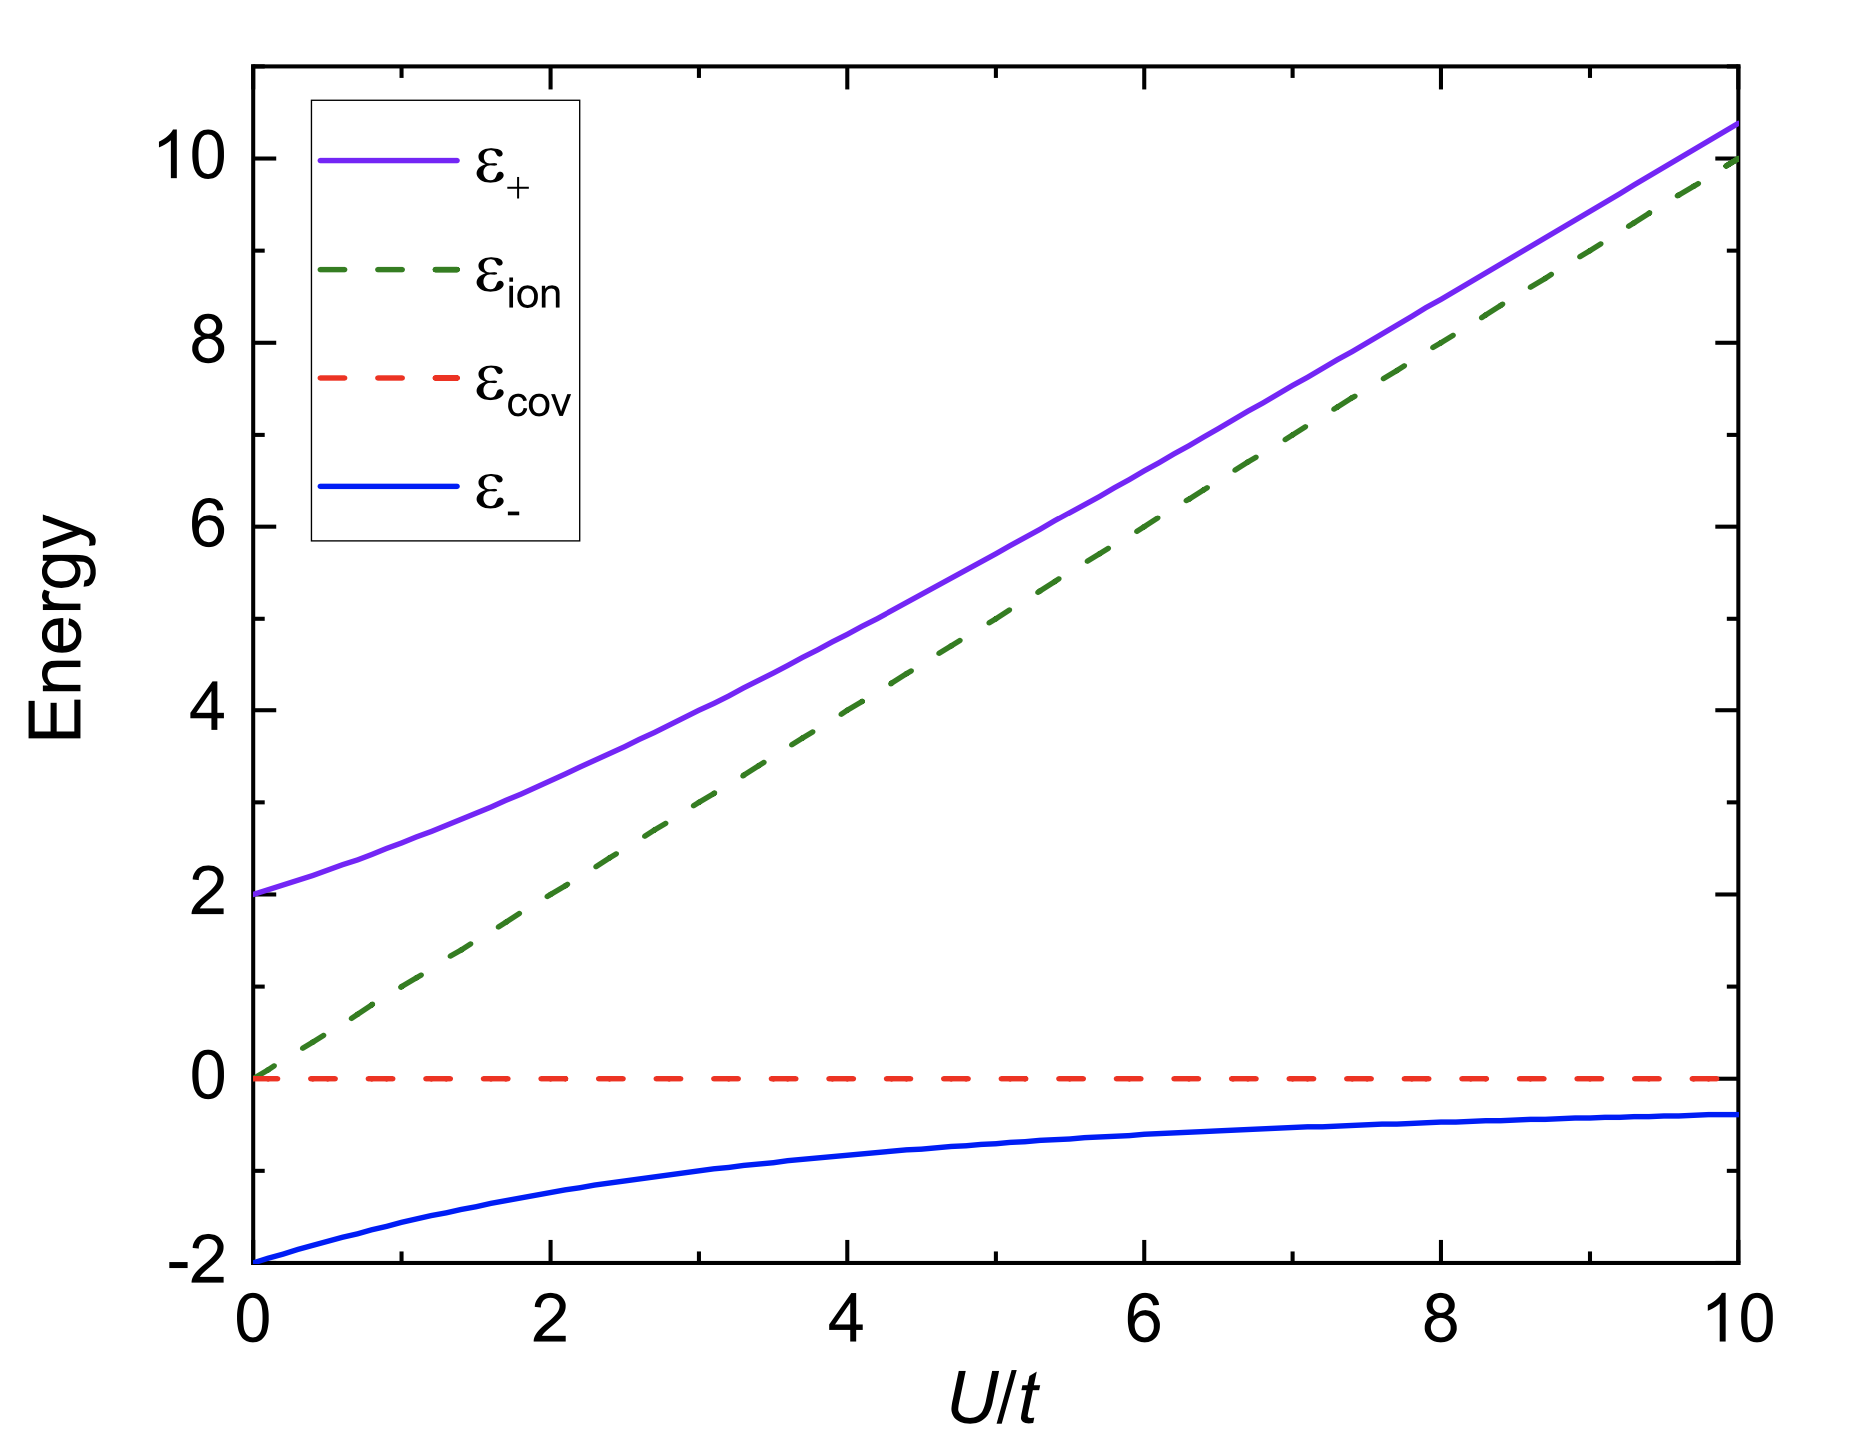
\includegraphics[width=0.8\textwidth]{figure/KE.png}
    \end{figure}
  \end{frame}
  %======================================================================

  %======================================================================
  \begin{frame}
    \frametitle{The 3rd method \(\blacktriangleright\) Kinetic exchange \(\blacktriangleright\) Downfolding}
    \footnotesize
    \begin{equation*}\scriptsize
      \widehat{H}_{t-U} = \begin{pmatrix}
        0 &  0 & -t & -t \;\\
        0 &  0 & +t & +t \;\\
       -t & +t &  U &  0 \;\\
       -t & +t &  0 &  U \;
      \end{pmatrix}\ \ \ \begin{matrix}
        |\uparrow\cdot,\downarrow\cdot\rangle\\
        |\downarrow\cdot,\uparrow\cdot\rangle\\
        |\uparrow\hspace{0.15em}\downarrow,\cdot\hspace{0.4em}\cdot\rangle\\
        |\hspace{0.1em}\cdot\hspace{0.15em}\cdot,\uparrow\hspace{0.15em}\downarrow\rangle
      \end{matrix}
    \end{equation*}
    If \(U \gg t\), then \(\widehat{H}_{11}\) can be regarded as a perturbation for \(\widehat{H}_{00}\).
    \begin{equation}
      \widehat{H}_{t-U} = \begin{pmatrix}
        \widehat{H}_{00} & \widehat{T}_{01}\\
        \widehat{T}_{10} & \widehat{H}_{11}
      \end{pmatrix}
    \end{equation}
    Use the downfolding technique\footnote{\tiny\url{https://diglib.tugraz.at/download.php?id=576a8c68b9df4&location=browse}}:
    \begin{subequations}
      \begin{align}
        \widehat{H}_{00}^{(\text{df})} &= \widehat{H}_{00} + \widehat{T}_{01}\left(\varepsilon\mathbb{1}-\widehat{H}_{11}\right)^{-1}\widehat{T}_{10}\\
        &\approx  \widehat{H}_{00} + \widehat{T}_{01}\left(\varepsilon_0\mathbb{1}-\widehat{H}_{11}\right)^{-1}\widehat{T}_{10}
      \end{align}
    \end{subequations}
    Where, \(\varepsilon\) is one eigenvalue of the selected (degenerated) subspace, and \(\varepsilon_0\) is the corresponding eigenvalue of \(\widehat{H}_{00}\).
  \end{frame}
  %======================================================================

  %======================================================================
  \begin{frame}
    \frametitle{The 3rd method \(\blacktriangleright\) Kinetic exchange \(\blacktriangleright\) Perturbation \(\widehat{H}_{\text{eff}}\)}
     Use the downfolding technique, we can get the perturbation Hamiltonian:
     \begin{equation}
      \begin{aligned}
        \widehat{H}_{\text{eff}} &= \begin{pmatrix}
          -t & -t \;\\
          +t & +t \;
        \end{pmatrix} \begin{pmatrix}
         \varepsilon-U & 0 \;\\
         0 & \varepsilon-U \;
        \end{pmatrix}^{-1} \begin{pmatrix}
         -t & +t \;\\
         -t & +t \;
        \end{pmatrix}\\
        &\approx -\dfrac{2t^2}{U}\begin{pmatrix}
          \phantom{+}1 & -1 \;\\
          -1 & \phantom{+}1 \;
        \end{pmatrix}
      \end{aligned}
     \end{equation}
     Diagonalizing the effective Hamiltonian, we find,
     \begin{subequations}
      \begin{align}
        &E_{\text{KS}} = -\dfrac{4t^2}{U},\ \ \Psi_{\text{S}} =  \frac{1}{\sqrt{2}}(|\uparrow\cdot,\downarrow\cdot\rangle - |\downarrow\cdot,\uparrow\cdot\rangle)\\
        &E_{\text{KT}} = 0, \hspace{2.4em}\Psi_{\text{T}} =  \frac{1}{\sqrt{2}}(|\uparrow\cdot,\downarrow\cdot\rangle + |\downarrow\cdot,\uparrow\cdot\rangle)
      \end{align}
     \end{subequations}
     For the other spin triplet (spin parallel) state, their kinetic energy also equal to \(0\).
  \end{frame}
  %======================================================================

  %======================================================================
  \begin{frame}
    \frametitle{The 3rd method \(\blacktriangleright\) Energy difference}
    \begin{table}
      \begin{tabular}{l|rrr}
        \hline
        \hline
       Item &Singlet&Triplet& \(E_\text{T}-E_\text{S}\)\\
        \hline
        Coulomb exchange&\(U_{ab}+J_{ab}\)&\(U_{ab}-J_{ab}\)& \(-2J_{ab}\)\\
        Kinetic exchange&\(-4t^2/U\)&\(0\)&\(4t^2/U\)\\
        Total & \(U_{ab}+J_{ab}-4t^2/U\)& \(U_{ab}-J_{ab}\)& \textcolor{purple}{\(-2J_{ab}+4t^2/U\)}\\
        \hline
        \hline
      \end{tabular}
    \end{table}
    \begin{block}{Observations}
      \begin{itemize}
        \item The result agree with what we find in the second method.
        \item Spin triplet states are degenerated on the Coulomb exchange term \item Spin triplet states are degenerated on the kinetic exchange term.
        \item \textcolor{purple}{Normally, the Coulomb exchange between different atomic site is very weak, for this term is only determined by the drirct overlap of orbits.}
        \item \textcolor{purple}{But, the kinetic exchange may not equally weak, for it can also come from ``indirect'' overlap.}
      \end{itemize}
    \end{block}
  \end{frame}
  %======================================================================

  \section{Different Exchange Type}

  %======================================================================
  \begin{frame}
    \frametitle{Exchange type}
    Since the Coulomb exchange between different atomic site is weak, when talking about the magnetism of a real material, we usually just focus on the kinetic exchange. Based on that, few difference exchange type is defined.
    \begin{block}{Exchange type}
      \begin{itemize}
        \item Direct exchange (direct overlap, kinetic energy)
        \item Superexchange (indirect overlap, kinetic energy)
        \item Super-superexchange (indirect overlap, kinetic energy)
        \item Double exchange (direct overlap, Coulomb energy \& kinetic energy)
      \end{itemize}
    \end{block}
  \end{frame}
  %======================================================================

  %======================================================================
  \begin{frame}
    \frametitle{Direct exchange}\footnotesize
    The Hamiltonian for direct exchange can be written as:
    \begin{equation*}
      \widehat{H}_{\text{dex}} = \begin{pmatrix}
        0 &  0 & -t & -t \;\\[0.2em]
        0 &  0 & +t & +t \;\\[0.2em]
       -t & +t &  U &  0 \;\\[0.2em]
       -t & +t &  0 &  U \;
      \end{pmatrix}\ \ \ \begin{matrix}
        \widehat{c}_{2\downarrow}^{\;\dagger}\widehat{c}_{1\uparrow}^{\;\dagger}|0\rangle\\
        \widehat{c}_{2\uparrow}^{\;\dagger}\widehat{c}_{1\downarrow}^{\;\dagger}|0\rangle\\
        \widehat{c}_{1\downarrow}^{\;\dagger}\widehat{c}_{1\uparrow}^{\;\dagger}|0\rangle\\
        \widehat{c}_{2\downarrow}^{\;\dagger}\widehat{c}_{2\uparrow}^{\;\dagger}|0\rangle\\
      \end{matrix}
    \end{equation*}
    After downfolding, 
    \begin{equation}
      \begin{aligned}
        \widehat{H}_{\text{dex}} &\approx -\dfrac{2t^2}{U}\begin{pmatrix}
          \phantom{+}1 & -1 \;\\
          -1 & \phantom{+}1 \;
        \end{pmatrix}\ \ \ \begin{matrix}
          \widehat{c}_{2\downarrow}^{\;\dagger}\widehat{c}_{1\uparrow}^{\;\dagger}|0\rangle\\
          \widehat{c}_{2\uparrow}^{\;\dagger}\widehat{c}_{1\downarrow}^{\;\dagger}|0\rangle
        \end{matrix}\\
        &= -\dfrac{2t^2}{U}\left(\widehat{c}_{1\downarrow}^{\;\dagger}\widehat{c}_{1\downarrow}\widehat{c}_{2\uparrow}^{\;\dagger}\widehat{c}_{2\uparrow} - \widehat{c}_{1\uparrow}^{\;\dagger}\widehat{c}_{1\downarrow}\widehat{c}_{2\downarrow}^{\;\dagger}\widehat{c}_{2\uparrow} - \widehat{c}_{1\downarrow}^{\;\dagger}\widehat{c}_{1\uparrow}\widehat{c}_{2\uparrow}^{\;\dagger}\widehat{c}_{2\downarrow}+\widehat{c}_{1\uparrow}^{\;\dagger}\widehat{c}_{1\uparrow}\widehat{c}_{2\downarrow}^{\;\dagger}\widehat{c}_{2\downarrow}\right)\\
        &= \dfrac{4t^2}{U} \left(\widehat{\bm{s}}_1\cdot\widehat{\bm{s}}_2 - \dfrac{\widehat{n}_1\widehat{n}_2}{4}\right) \sim \dfrac{4t^2}{U} \widehat{\bm{s}}_1\cdot\widehat{\bm{s}}_2
      \end{aligned} 
    \end{equation}
    Where, for electron spin \(\widehat{\bm{s}}_i = (\widehat{s}_{ix},\widehat{s}_{iy},\widehat{s}_{iz})\):
    \begin{equation}
      \widehat{s}_{ix} = \dfrac{1}{2}\left(\widehat{c}_{i\uparrow}^{\;\dagger}\widehat{c}_{i\downarrow}+\widehat{c}_{i\downarrow}^{\;\dagger}\widehat{c}_{i\uparrow}\right),\ \ 
      \widehat{s}_{iy} = -\dfrac{i}{2}\left(\widehat{c}_{i\uparrow}^{\;\dagger}\widehat{c}_{i\downarrow}-\widehat{c}_{i\downarrow}^{\;\dagger}\widehat{c}_{i\uparrow}\right),\ \ 
      \widehat{s}_{iz} = \dfrac{1}{2}\left(\widehat{n}_{i\uparrow} - \widehat{n}_{i\downarrow}\right)
    \end{equation}
  \end{frame}
  %======================================================================

  %======================================================================
  \begin{frame}
    \frametitle{Superexchange}
    \begin{figure}
      \centering
      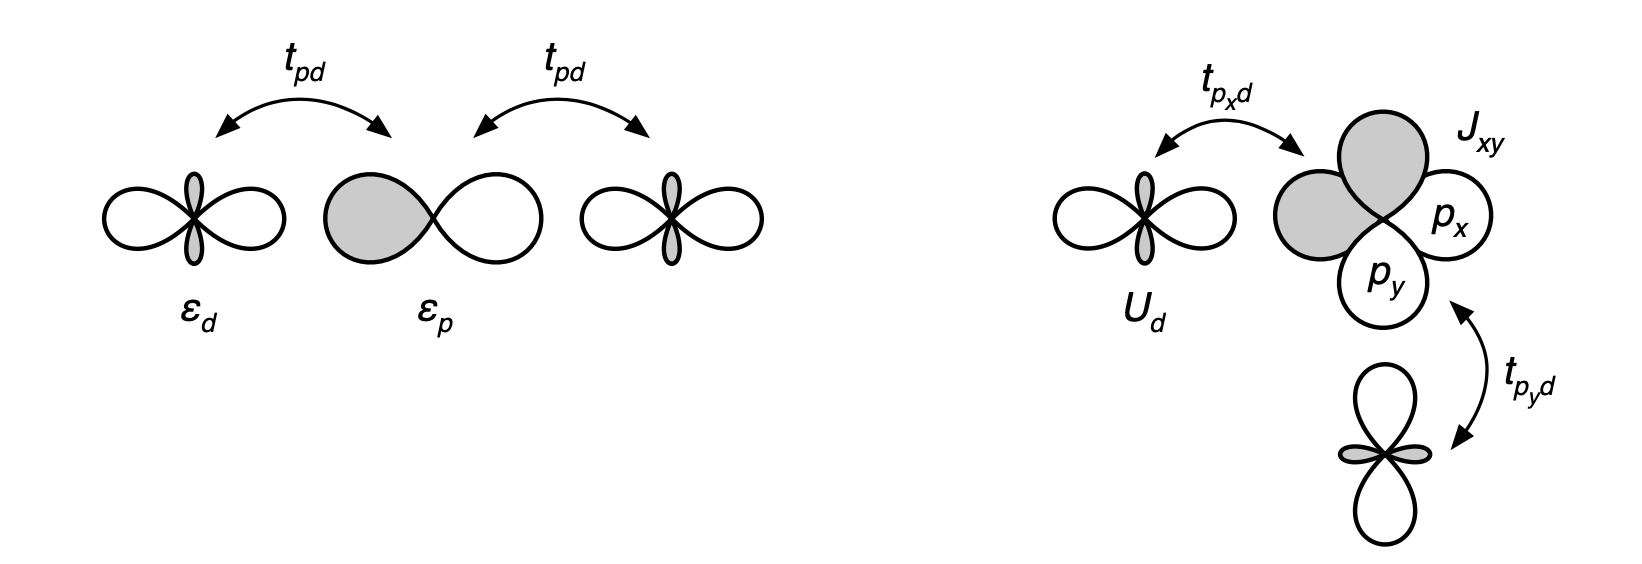
\includegraphics[width=\textwidth]{figure/SupEx.png}
    \end{figure}
    \begin{block}{Notes}
      \begin{itemize}
        \item The \(180^{\circ}\) superexchange prefer AFM. 
        \item The \(90^{\circ}\) superexchange prefer FM. 
      \end{itemize}
    \end{block}
    \textcolor{gray}{Remember, we are still discussing the ``two spin sites model'' now.}
  \end{frame}
  %======================================================================

  %======================================================================
  \begin{frame}
    \frametitle{\(180^{\circ}\) superexchange \(\blacktriangleright\) Hubbard Hamiltonian}\footnotesize
    The Hamiltonian for \(180^{\circ}\) superexchange can be written as:
    \begin{equation}
      \widehat{H}_{\text{sup}} = \sum_{\sigma} \left(\varepsilon_d\sum_{i=1,2}\widehat{n}_{i\sigma}+\varepsilon_p\widehat{n}_{p\sigma}-t_{pd}\sum_{i=1,2}\left(\widehat{c}_{i\sigma}^{\;\dagger}\widehat{c}_{p\sigma}+\widehat{c}_{p\sigma}^{\;\dagger}\widehat{c}_{i\sigma}\right)\right) + U_d \sum_{i=1,2}\widehat{n}_{i\uparrow}\widehat{n}_{i\downarrow}
    \end{equation}
    The figure below will show us how to select the projection basis.
    \begin{figure}
      \centering 
      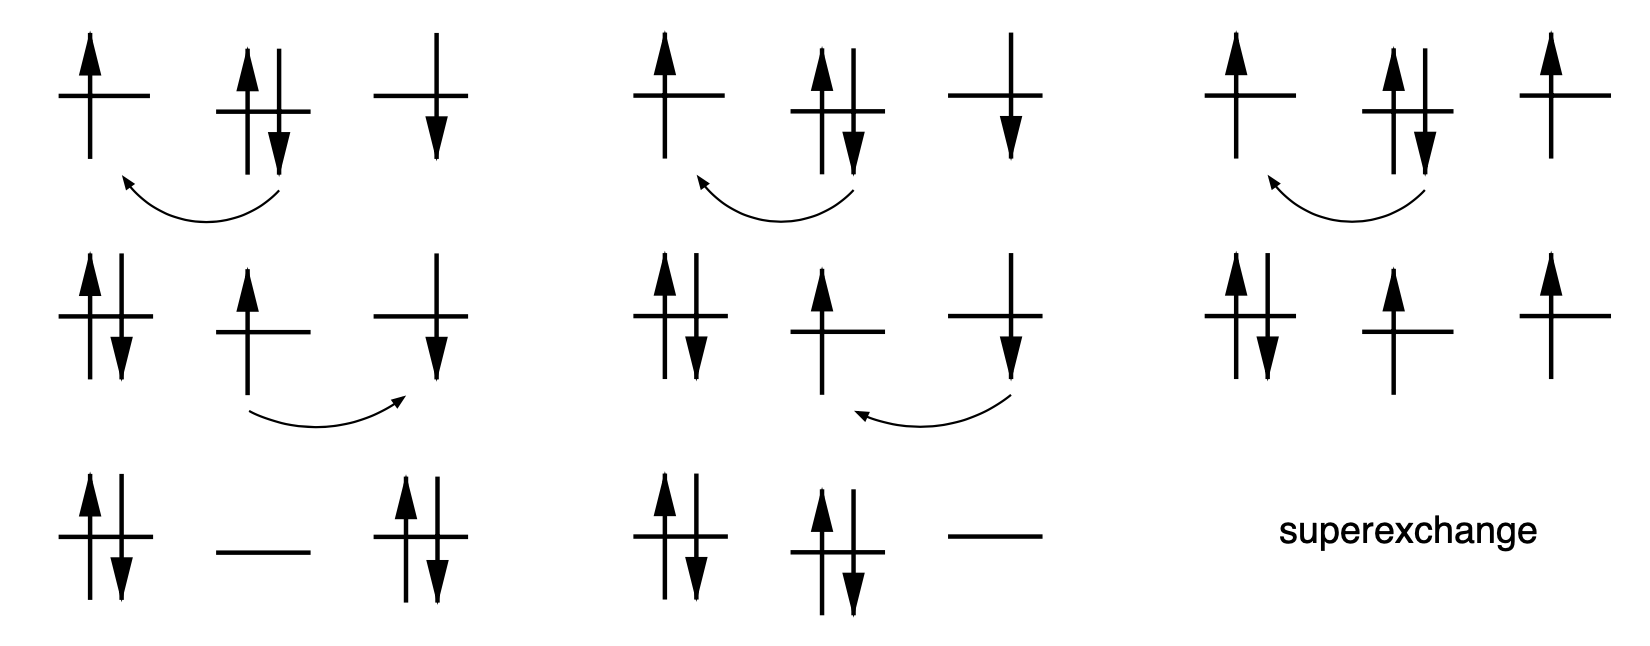
\includegraphics[width=0.9\textwidth]{figure/180-supex-basis.png}
    \end{figure}
  \end{frame}
  %======================================================================

  %======================================================================
  \begin{frame}
    \frametitle{\(180^{\circ}\) superexchange \(\blacktriangleright\) Spin parallel}
    For the spin parallel subspace:
    \begin{equation}
      \widehat{H}_{\text{sup}} = \begin{pmatrix}\begin{array}{c|cc}
        0 & t_{pd} & t_{pd}\\[0.5em]\hline
        t_{pd} & U_d + \Delta_{pd} & 0 \\[0.5em]
        t_{pd} & 0 & U_d + \Delta_{pd}
      \end{array}\end{pmatrix}\ \ \ \begin{matrix}
        \widehat{c}_{2\uparrow}^{\;\dagger}\widehat{c}_{p\downarrow}^{\;\dagger}\widehat{c}_{p\uparrow}^{\;\dagger}\widehat{c}_{1\uparrow}^{\;\dagger}|0\rangle\\
        \widehat{c}_{2\uparrow}^{\;\dagger}\widehat{c}_{p\uparrow}^{\;\dagger}\widehat{c}_{1\downarrow}^{\;\dagger}\widehat{c}_{1\uparrow}^{\;\dagger}|0\rangle\\
        \widehat{c}_{2\downarrow}^{\;\dagger}\widehat{c}_{p\uparrow}^{\;\dagger}\widehat{c}_{p\uparrow}^{\;\dagger}\widehat{c}_{1\uparrow}^{\;\dagger}|0\rangle
      \end{matrix}
    \end{equation}
    Where, \(\Delta_{pd} = \varepsilon_d - \varepsilon_p\).

    Using downfolding technique,
    \begin{equation}
      \begin{aligned}
        \widehat{H}_{\text{sup}} &= (t_{pd}, t_{pd})\begin{pmatrix}
          \varepsilon-(U_d + \Delta_{pd}) & 0\\
          0 & \varepsilon-(U_d + \Delta_{pd})
        \end{pmatrix}^{-1}\begin{pmatrix}
          t_{pd}\\
          t_{pd}
        \end{pmatrix}\\
        &\approx-\dfrac{2t_{pd}}{U_d} + \Delta_{pd}
      \end{aligned}
    \end{equation}
  \end{frame}
  %======================================================================

  %======================================================================
  \begin{frame}
    \frametitle{\(180^{\circ}\) superexchange \(\blacktriangleright\) Spin anti-parallel}\footnotesize
    For the spin anti-parallel subspace:
    \begin{equation}\arraycolsep=0.2pt
      \widehat{H}_{\text{sup}} = \begin{pmatrix}\tiny\begin{array}{cc|cccc|ccc}
        0 & 0 & +t_{pd} & +t_{pd} & 0 & 0 & 0 & 0 & 0\\[0.5em]
        0 & 0 & 0 & 0 & +t_{pd} & +t_{pd} &0 & 0 & 0 \\[0.5em]\hline
        +t_{pd} & 0 & U_d+\Delta_{pd} & 0 & 0 & 0 & -t_{pd} & 0 & -t_{pd}\\[0.5em]
        +t_{pd} & 0 & 0 & U_d+\Delta_{pd} & 0 & 0 & 0 & -t_{pd} & -t_{pd}\\[0.5em]
        0 & +t_{pd} & 0 & 0 & U_d+\Delta_{pd} & 0 & +t_{pd} & 0 & +t_{pd}\\[0.5em]
        0 & +t_{pd} & 0 & 0 & 0 & U_d+\Delta_{pd} & 0 & +t_{pd} & +t_{pd}\\[0.5em]\hline
        0 & 0 & -t_{pd} & 0 & +t_{pd} & 0 & U_d & 0 & 0\\[0.5em]
        0 & 0 & 0 & -t_{pd} & 0 & +t_{pd} & 0 & U_d & 0\\[0.5em]
        0 & 0 & -t_{pd} & -t_{pd} & +t_{pd} & +t_{pd} & 0 & 0 & 2(U_d+\Delta_{pd})
      \end{array}\end{pmatrix}\ \ \ \begin{matrix}\tiny\begin{array}{c}
        \widehat{c}_{2\downarrow}^{\;\dagger}\widehat{c}_{p\downarrow}^{\;\dagger}\widehat{c}_{p\uparrow}^{\;\dagger}\widehat{c}_{1\uparrow}^{\;\dagger}|0\rangle\\
        \widehat{c}_{2\uparrow}^{\;\dagger}\widehat{c}_{p\downarrow}^{\;\dagger}\widehat{c}_{p\uparrow}^{\;\dagger}\widehat{c}_{1\downarrow}^{\;\dagger}|0\rangle\\
        \widehat{c}_{2\uparrow}^{\;\dagger}\widehat{c}_{p\uparrow}^{\;\dagger}\widehat{c}_{1\downarrow}^{\;\dagger}\widehat{c}_{1\uparrow}^{\;\dagger}|0\rangle\\
        \widehat{c}_{2\downarrow}^{\;\dagger}\widehat{c}_{2\uparrow}^{\;\dagger}\widehat{c}_{p\downarrow}^{\;\dagger}\widehat{c}_{1\uparrow}^{\;\dagger}|0\rangle\\
        \widehat{c}_{2\uparrow}^{\;\dagger}\widehat{c}_{p\downarrow}^{\;\dagger}\widehat{c}_{1\downarrow}^{\;\dagger}\widehat{c}_{1\uparrow}^{\;\dagger}|0\rangle\\
        \widehat{c}_{2\downarrow}^{\;\dagger}\widehat{c}_{2\uparrow}^{\;\dagger}\widehat{c}_{p\uparrow}^{\;\dagger}\widehat{c}_{1\downarrow}^{\;\dagger}|0\rangle\\
        \widehat{c}_{p\downarrow}^{\;\dagger}\widehat{c}_{p\uparrow}^{\;\dagger}\widehat{c}_{1\downarrow}^{\;\dagger}\widehat{c}_{1\uparrow}^{\;\dagger}|0\rangle\\
        \widehat{c}_{2\downarrow}^{\;\dagger}\widehat{c}_{2\uparrow}^{\;\dagger}\widehat{c}_{p\downarrow}^{\;\dagger}\widehat{c}_{p\uparrow}^{\;\dagger}|0\rangle\\
        \widehat{c}_{2\downarrow}^{\;\dagger}\widehat{c}_{2\uparrow}^{\;\dagger}\widehat{c}_{1\downarrow}^{\;\dagger}\widehat{c}_{1\uparrow}^{\;\dagger}|0\rangle
      \end{array}\end{matrix}
    \end{equation}
    Using downfolding technique,
    \begin{equation}
      \begin{aligned}
        \widehat{H}_{\text{sup}} &= \widehat{H}_{00} + \widehat{T}_{01}(\varepsilon - (\widehat{H}_{11}+\widehat{T}_{12}(\varepsilon-\widehat{H}_{22})^{-1}\widehat{T}_{21}))^{-1}\widehat{T}_{10}\\
        &\approx \widehat{H}_{00} - \widehat{T}_{01}\widehat{H}_{11}^{-1}\widehat{T}_{10} - \widehat{T}_{01}\widehat{H}_{11}^{-1}\widehat{T}_{12}\widehat{H}_{22}^{-1}\widehat{T}_{21}\widehat{T}_{10}\\
        &= -\dfrac{2t_{pd}^2}{U_d + \Delta_{pd}}\begin{pmatrix}
          1 & 0\\
          0 & 1
        \end{pmatrix} - \dfrac{2t^4_{pd}}{(U_d+\Delta_{pd})^2}\left(\dfrac{1}{U_d} + \dfrac{1}{U_d+\Delta_{pd}}\right)\begin{pmatrix}
          \phantom{+}1 & -1\\
          -1 & \phantom{+}1
        \end{pmatrix}\\
        &\xlongequal{diag.}-\dfrac{2t_{pd}^2}{U_d + \Delta_{pd}}\begin{pmatrix}
          1 & 0\\
          0 & 1
        \end{pmatrix} - \dfrac{4t^4_{pd}}{(U_d+\Delta_{pd})^2}\left(\dfrac{1}{U_d} + \dfrac{1}{U_d+\Delta_{pd}}\right)\begin{pmatrix}
          1 & 0\\
          0 & 0
        \end{pmatrix}
      \end{aligned}
    \end{equation}
  \end{frame}
  %======================================================================

  %======================================================================
  \begin{frame}
    \frametitle{\(180^{\circ}\) superexchange \(\blacktriangleright\) Effective Hamiltonian}\footnotesize
    The spin parallel state Hamiltonian is:
    \begin{equation}
      \widehat{H}_{\text{par}} = -\dfrac{2t_{pd}^2}{U_d + \Delta_{pd}}\begin{pmatrix}
        1 & 0\\
        0 & 1
      \end{pmatrix}
    \end{equation}

    The spin anti-parallel state Hamiltonian is:
    \begin{equation}
      \widehat{H}_{\text{apar}} = -\dfrac{2t_{pd}^2}{U_d + \Delta_{pd}}\begin{pmatrix}
        1&0\\
        0&1
      \end{pmatrix} - \dfrac{4t^4_{pd}}{(U_d+\Delta_{pd})^2}\left(\dfrac{1}{U_d} + \dfrac{1}{U_d+\Delta_{pd}}\right)\begin{pmatrix}
        1 & 0\\
        0 & 0
      \end{pmatrix}
    \end{equation}

    So, the energy difference between spin singlet and triplet state is:
    \begin{equation}
      E_\text{T} - E_\text{S} = \dfrac{4t^4_{pd}}{(U_d+\Delta_{pd})^2}\left(\dfrac{1}{U_d} + \dfrac{1}{U_d+\Delta_{pd}}\right)
    \end{equation}

    Or, we can use the relation between \(\widehat{\bm{s}_i}\) and \(\widehat{c}_i\) to get the effective Hamiltonian:
    \begin{equation}
      \widehat{H}_{\text{sup}} = \dfrac{4t^4_{pd}}{(U_d+\Delta_{pd})^2}\left(\dfrac{1}{U_d} + \dfrac{1}{U_d+\Delta_{pd}}\right) \widehat{\bm{s}}_1 \cdot \widehat{\bm{s}}_2
    \end{equation}

    The \(180^{\circ}\) superexchange prefer AFM. \qed
  \end{frame}
  %======================================================================

  %======================================================================
  \begin{frame}
    \frametitle{\(90^{\circ}\) superexchange \(\blacktriangleright\) Effective Hamiltonian}
    \begin{block}{Basic step to obtain the effective Hamiltonian}
      \begin{itemize}
        \item Write the original Hamiltonian. (Hubbard model)
        \item Draw all the related spin state.
        \item Confirm the basis.
        \item Project the Hamiltonian on the basis.
        \item Downfolding.
        \item Use the relation between \(\widehat{\bm{s}_i}\) and \(\widehat{c}_i\) to get the effective Hamiltonian
      \end{itemize}
    \end{block}
    The effective Hamiltonian for \(90^{\circ}\) superexchange is:
    \begin{equation}
      \widehat{H}_{\text{sup}} = -\dfrac{4t_4}{(U_d+\Delta_{pd})^2} \dfrac{2J_{xy}}{4(U_d+\Delta_{pd})^2-J^2_{xy}}\widehat{\bm{s}}_1 \cdot \widehat{\bm{s}}_2
    \end{equation}
    Where, \(J_{xy}\) is the Coulomb exchange between orbit \(p_x\) and \(p_y\).

    \(90^{\circ}\) superexchange prefer FM.
  \end{frame}
  %======================================================================

  \section{Multiple electrons system}

  %======================================================================
  \begin{frame}
    \frametitle{Heisenberg exchange model for multiple electrons}
    For spin two sites model, the Heisenberg Hamiltonian is:
    \begin{equation*}
      \widehat{H}_{A\text{d}} = -2A\;\widehat{\bm{s}}_1\cdot\widehat{\bm{s}}_2
    \end{equation*}
    When system having more that two sites (still one electron each site), the Heisenberg Hamiltonian is:
    \begin{equation}
        \widehat{H}_A = -\sum_{i\ne{}j}A_{ij}\widehat{\bm{s}}_i\cdot\widehat{\bm{s}}_j
    \end{equation}
    
    For each pair of sites, the analysis is the same as before. 

    Further more, the formula is the same, if there are more than one electron on each site, e.g.\(3d^6\).
    \begin{block}{Multiple electrons Heisenberg Hamiltonian}
      \begin{equation}
        \widehat{H} = -\sum_{i\ne{}j}A_{ij}\widehat{\bm{S}}_i\cdot\widehat{\bm{S}}_j = \dfrac{1}{2}\sum_{i\ne{}j}J_{ij}\widehat{\bm{S}}_i\cdot\widehat{\bm{S}}_j
      \end{equation}
      Where, the \(\widehat{\bm{S}}_i, \widehat{\bm{S}}_j\) is determined by the Hund's rule.
    \end{block}
  \end{frame}
  %======================================================================

  %======================================================================
  \begin{frame}
    \frametitle{Applications of Heisenberg model}
    \begin{equation*}
      \widehat{H} = -\sum_{i\ne{}j}A_{ij}\widehat{\bm{S}}_i\cdot\widehat{\bm{S}}_j = \dfrac{1}{2}\sum_{i\ne{}j}J_{ij}\widehat{\bm{S}}_i\cdot\widehat{\bm{S}}_j
    \end{equation*}
    \begin{block}{Application}
      Using the Hamiltonian above, we can describe:
    \begin{itemize}
      \item Integer magnetic moment below \(T_\text{C}\). (Weiss molecular field)
      \begin{itemize}
        \item Magnetism in 3d-oxides. (Anderson model, or kinetic exchange)
        \item Magnetism in 4f elements or GMR. (RKKY)
      \end{itemize}
      \item Magnetism near \(T_\text{C}\) (Oguchi theory, BPW method).
      \item Magnetism near 0K, magnon. (Holstein–Primakoff transformation)
    \end{itemize}
    We cannot describe:
    \begin{itemize}
      \item Fractional magnetic moment below \(T_\text{C}\). 
    \end{itemize}
    \end{block}
  \end{frame}
  %======================================================================

  %======================================================================
  \begin{frame}
    \frametitle{Magnetic analysis of multiple electrons system}
    When discussing Heisenberg Hamiltonian for multiple electrons, we can (using Hund's rule) \textcolor{purple}{add up all the spin} around the same atom. But when analysing the origin of its magnetic, we still need to use the \textcolor{purple}{picture of single electron hopping}.
    \begin{equation*}
      \begin{matrix}
      \downarrow&\overline{\hspace{1em}}\;\overline{\hspace{1em}}\ \ &\ \  \overline{\hspace{1em}}\;\overline{\hspace{1em}}\\
      \uparrow&\overline{\hspace{1em}}\;\overline{\hspace{1em}}\ \ &\ \  \overline{\hspace{1em}}\;\overline{\hspace{1em}}\\[0.6em]
      \downarrow&\overline{\hspace{1em}}\;\overline{\hspace{1em}}\;\overline{\hspace{1em}}\ \ &\ \  \overline{\hspace{1em}}\;\overline{\hspace{1em}}\;\overline{\hspace{1em}}\\
      \uparrow&\overline{\hspace{1em}}\;\overline{\hspace{1em}}\;\overline{\hspace{1em}}\ \ &\ \  \overline{\hspace{1em}}\;\overline{\hspace{1em}}\;\overline{\hspace{1em}}\\[0.6em]
      3d &\text{Atom1} & \text{Atom2}
      \end{matrix}
    \end{equation*}
  \end{frame}
  %======================================================================

  %======================================================================
  \begin{frame}
    \frametitle{Magnetic analysis of multiple electrons system}
    \begin{block}{Bacis info.}
      In order to perform a qualitative analysis about the magnetic of a specific material, we need some basic information:
      \begin{itemize}
        \item Crystal field split (symmetry analysing)
        \item Spin split (band analysing)
        \item Electrons filling (valence analysing)
        \item Hopping path (bonding and orbital analysing)
        \item MAE \textcolor{gray}{(not discussed yet...)}
      \end{itemize}
    \end{block}
    \textcolor{gray}{The Coulomb exchange is usually ignored, if not in a double exchange analysing.}
  \end{frame}
  %======================================================================

  %======================================================================
  \begin{frame}
    \frametitle{Goodenough-Kanamori rules}
    \begin{block}{Goodenough-Kanamori rules}
      \begin{enumerate}
      \item When two cations have lobes of singly occupied \(3d\)-orbitals which point towards each other giving large overlap and hopping intergrals, the exchange is strong and antiferromagnetic (\(J<0\)). This is the usual case, for \(120^{\circ}-180^{\circ}\) M-O-M bonds.

      \item When two cations have a overlap integral between singly occupied \(3d\)-orbitals which is zero by symmetry, the exchange is ferromagnetic and relatively	weak. This is the case for \(\sim 90^{\circ}\) M-O-M bonds.

      \item When two cations have an overlap between singly occupied 3d orbitals and empty or doubly occupied orbitals of the same type, the exchange is also ferromagnetic, and relatively weak.
      \end{enumerate}
    \end{block}
    The Goodenough-Kanamori rules are semiempirical rules. It can be derived from the kinetic hopping picture, and works well in practice.
  \end{frame}
  %======================================================================

  \section{Summary}

  %======================================================================
  \begin{frame}
    \frametitle{Summary}
    \begin{block}{Summary}
      \begin{itemize}
        \item The magnetic order is related to the spin triplet and singlet state.
        \item Under the electronic exchange interaction, the 4 degenerated spin state split into 1 spin singlet state and 3 spin triplet state.
        \item The exchange interaction can be divided into Coulomb exchange and kinetic exchange. The latter is usually more important.
        \item The Coulomb exchange always prefer FM, while the kinetic exchange depends on the situation.
        \item Downfolding is an effective technique to carry the energy perturbation.
        \item Using the hopping picture, we can explain most of the 
        magnetism in insulators.
        \item Goodenough-Kanamori rules is a handy tool in determine the sign of kinetic exchange.
      \end{itemize}
    \end{block}
  \end{frame}
  %======================================================================

  %======================================================================
  \begin{frame}
    \frametitle{Additional notes}
    \begin{block}{Notes}
      \begin{itemize}
        \item In DFT calculation, the energy splitting of the up-spin and down-spin can be simulated by DFT+\(U\) or hybrid functional method.
        \item The orbit magnetization is not counted for it is not appear in the effective Hamiltonian. Only after considering the SOC, will the orbit term show.
        \item The Heisenberg Hamiltonian is a effective model. Once we find the energy difference between the spin triplet and singlet state (no matter caused by what), we can use the Heisenberg model to describe all of the magnetic properties.
      \end{itemize}
    \end{block}
    The more general spin Hamiltonian for magnetic.
    \begin{equation}\scriptsize
      \widehat{H}_{\text{mag}} = \dfrac{1}{2}\sum_{i\ne{}j}J_{ij}\widehat{\bm{S}}_i\cdot\widehat{\bm{S}}_j + \dfrac{1}{2}\sum_{i\ne{}j}\bm{D}_{ij}\cdot\left(\widehat{\bm{S}}_i\times\widehat{\bm{S}}_j\right) + \sum_i A_i\widehat{S}_{iz}^2 + \dfrac{1}{2}\sum_{i\ne{}j}K_{ij}\left(\widehat{\bm{S}}_i\cdot\widehat{\bm{S}}_j\right)^2
    \end{equation}
  \end{frame}
  %======================================================================

\end{document} 